\documentclass[tikz,border=4pt]{standalone}

\usetikzlibrary{positioning,arrows.meta,fit,backgrounds}

\tikzset{
  font=\sffamily,
  split/.style={draw, rounded corners, inner sep=.45em, fill=blue!15},
  leaf/.style={draw, rounded corners, inner sep=.45em, fill=green!15},
  unit/.style={draw, circle, minimum size=2.2em, inner sep=0pt},
  edgelbl/.style={font=\sffamily\scriptsize, inner sep=1pt},
  arrow/.style={-{Stealth[length=2mm]}},
  wpos/.style={arrow, thick},
  wneg/.style={arrow, thick, dashed},
}

\begin{document}
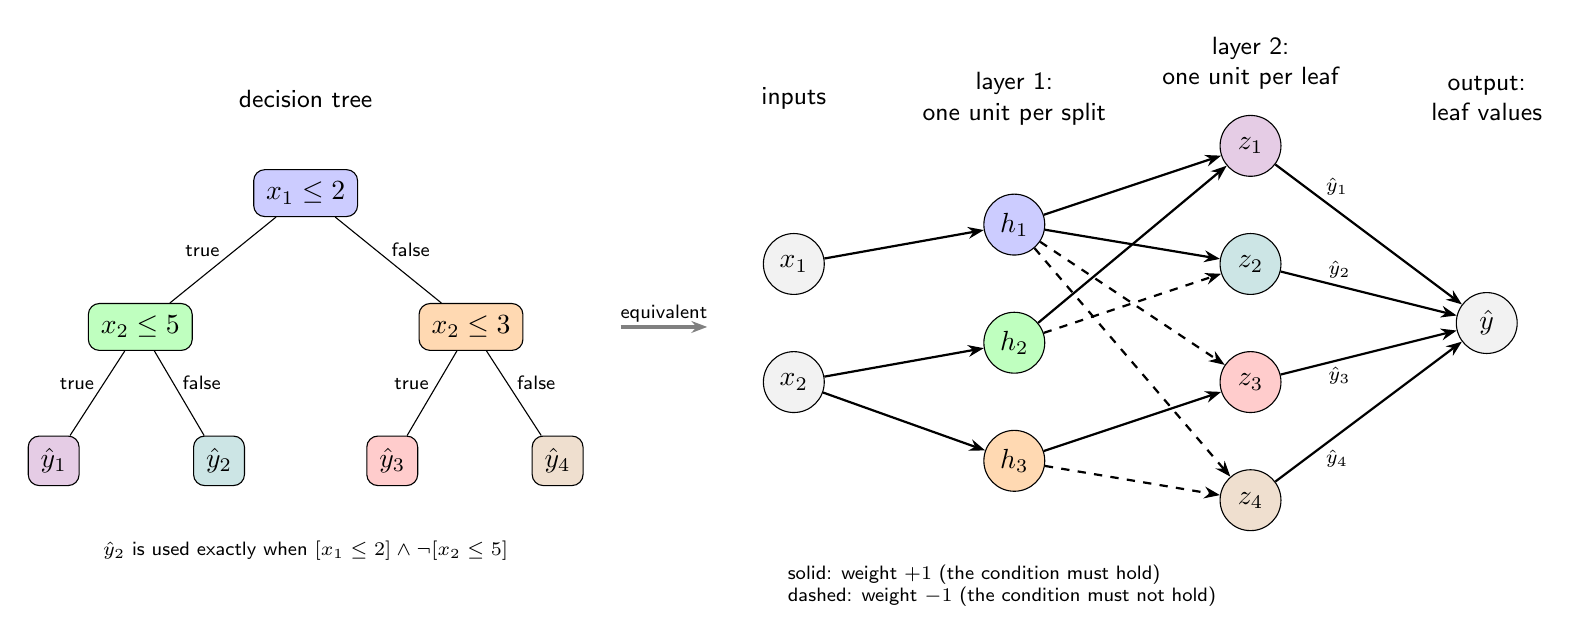
\begin{tikzpicture}[x=1cm, y=1cm]

  % ---------------- the decision tree ----------------
  \node[split, fill=blue!20]   (t1) at (0, 0)      {$x_1 \le 2$};
  \node[split, fill=green!25]  (t2) at (-2.1, -1.7) {$x_2 \le 5$};
  \node[split, fill=orange!30] (t3) at (2.1, -1.7)  {$x_2 \le 3$};
  \node[leaf, fill=violet!20] (l1) at (-3.2, -3.4) {$\hat y_1$};
  \node[leaf, fill=teal!20]   (l2) at (-1.1, -3.4) {$\hat y_2$};
  \node[leaf, fill=red!20]    (l3) at (1.1, -3.4)  {$\hat y_3$};
  \node[leaf, fill=brown!25]  (l4) at (3.2, -3.4)  {$\hat y_4$};

  \draw (t1) -- node[edgelbl, above left] {true} (t2);
  \draw (t1) -- node[edgelbl, above right] {false} (t3);
  \draw (t2) -- node[edgelbl, above left] {true} (l1);
  \draw (t2) -- node[edgelbl, above right] {false} (l2);
  \draw (t3) -- node[edgelbl, above left] {true} (l3);
  \draw (t3) -- node[edgelbl, above right] {false} (l4);

  % ---------------- the network ----------------
  \node[unit, fill=gray!10] (x1) at (6.2, -0.9) {$x_1$};
  \node[unit, fill=gray!10] (x2) at (6.2, -2.4) {$x_2$};

  \node[unit, fill=blue!20]   (h1) at (9.0, -0.4) {$h_1$};
  \node[unit, fill=green!25]  (h2) at (9.0, -1.9) {$h_2$};
  \node[unit, fill=orange!30] (h3) at (9.0, -3.4) {$h_3$};

  \node[unit, fill=violet!20] (z1) at (12.0, 0.6)  {$z_1$};
  \node[unit, fill=teal!20]   (z2) at (12.0, -0.9) {$z_2$};
  \node[unit, fill=red!20]    (z3) at (12.0, -2.4) {$z_3$};
  \node[unit, fill=brown!25]  (z4) at (12.0, -3.9) {$z_4$};

  \node[unit, fill=gray!10] (out) at (15.0, -1.65) {$\hat y$};

  \draw[wpos] (x1) -- (h1);
  \draw[wpos] (x2) -- (h2);
  \draw[wpos] (x2) -- (h3);

  \draw[wpos] (h1) -- (z1);  \draw[wpos] (h2) -- (z1);
  \draw[wpos] (h1) -- (z2);  \draw[wneg] (h2) -- (z2);
  \draw[wneg] (h1) -- (z3);  \draw[wpos] (h3) -- (z3);
  \draw[wneg] (h1) -- (z4);  \draw[wneg] (h3) -- (z4);

  \draw[wpos] (z1) -- node[edgelbl, above right, pos=.25] {$\hat y_1$} (out);
  \draw[wpos] (z2) -- node[edgelbl, above right, pos=.25] {$\hat y_2$} (out);
  \draw[wpos] (z3) -- node[edgelbl, below right, pos=.25] {$\hat y_3$} (out);
  \draw[wpos] (z4) -- node[edgelbl, below right, pos=.25] {$\hat y_4$} (out);

  % ---------------- captions ----------------
  \node[font=\sffamily\small] at (0, 1.2) {decision tree};
  \node[font=\sffamily\small, align=center] at (6.2, 1.2) {inputs};
  \node[font=\sffamily\small, align=center] at (9.0, 1.2) {layer 1:\\one unit per split};
  \node[font=\sffamily\small, align=center] at (12.0, 1.65) {layer 2:\\one unit per leaf};
  \node[font=\sffamily\small, align=center] at (15.0, 1.2) {output:\\leaf values};

  \node[font=\sffamily\scriptsize, align=left, anchor=north west] at (6.0, -4.6)
    {solid: weight $+1$ (the condition must hold)\\dashed: weight $-1$ (the condition must not hold)};
  \node[font=\sffamily\scriptsize, align=center, anchor=north] at (0, -4.3)
    {$\hat y_2$ is used exactly when $[x_1 \le 2] \wedge \neg[x_2 \le 5]$};

  \draw[arrow, very thick, gray] (4.0, -1.7) -- node[edgelbl, above, text=black] {equivalent} (5.1, -1.7);
\end{tikzpicture}
\end{document}
